\documentclass[conference]{IEEEtran}
%\IEEEoverridecommandlockouts
% The preceding line is only needed to identify funding in the first footnote. If that is unneeded, please comment it out.
\usepackage{cite}
\usepackage{amsmath,amssymb,amsfonts}
\usepackage{algorithmic}
\usepackage{graphicx}
\usepackage{textcomp}
\usepackage{xcolor}
\def\BibTeX{{\rm B\kern-.05em{\sc i\kern-.025em b}\kern-.08em
    T\kern-.1667em\lower.7ex\hbox{E}\kern-.125emX}}
\begin{document}

\title{TLC5540 \\
}

\author{\IEEEauthorblockN{Nicholas Snyder}
\IEEEauthorblockA{\textit{Department of Electrical and Computer Engineering} \\
\textit{University of New Hampshire}\\
Durham, United States of America \\
Nick.Snyder@usnh.edu \\ 
18 December 2023}
}

\maketitle

\begin{abstract}

The TLC5540 is an 8-bit, high-speed analog-to-digital converter (ADC) that can operate at a sampling rate of up to 40 MSPS. It uses a semiflash architecture and CMOS process to achieve low power consumption and cost. This research paper evaluates the performance and accuracy of the TLC5540 ADC in terms of power efficiency, resolution, linearity, and noise. The paper also compares the TLC5540 ADC with other similar ADCs in the market and explores its potential applications in various fields, such as digital signal processing, data acquisition, and communication systems.

\end{abstract}

\section{Introduction}

An ADC is a critical component in all circuits where decoding analog signals are necessary to its funciton. An ADC's basic function is simply converting an analog signal to a digital signal of various resolutions using a collection of comparators and an encoder among others. There are many different types of ADCs for different levels of precision and complexity. \par
The TLC5540 in particular is a high-speed, 8-bit ADC that converts at sampling rates up to 40 megasamples per second (MSPS). Using a semiflash architecture and CMOS process, the TLC5540 is able to convert at high speeds while still maintaining low power consumption and cost. The analog input bandwidth of 75 MHz (typ) makes this device an excellent choice for undersampling applications. Internal resistors are provided to generate 2-V full-scale reference voltages from a 5-V supply, thereby reducing external components. The digital outputs can be placed in a high impedance mode. The TLC5540 requires only a single 5-V supply for operation \cite{b1}. \par
An ADC is used in applications where high precision is necessary. They can be found inside musical devices, scientific instrumentation, and displays. \par
The first ADCs to designed were at Bell Labs in the 1940s. Using vacuum tubes at the time, the successive approximation ADC were used in World War II to encrypt voice communications for the Allies \cite{b2}.

\section{Device Architechture}

The symbol of a common ADC has a pointed end on the left side input and a square face on the right side output. Fig. 1. clearly indicates which end is the input and which is the output.

\begin{figure}[htbp]
\centerline{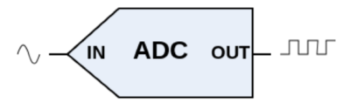
\includegraphics{ADCsym.png}}
\caption{Symbol of a common ADC.}
\end{figure}

Due to the precise nature of the TLC5540, it is quite complex under the hood. As seen in Fig. 2., the packadge contains a resistance reference divider circuit, a clock generator, upper and lower sampling comparators, upper and lower encoders, and upper and lower data latches.

\begin{figure}[htbp]
\centerline{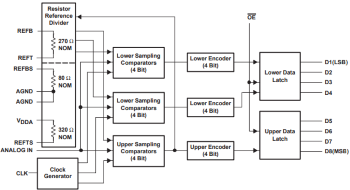
\includegraphics{ADCblkTI.png}}
\caption{Function block diagram of TLC5540 ADC.}
\end{figure}

There are many different kinds of ADCs for different applications where different levels of precision, cost, and power draw are taken into consideration. A simple ADC like Flash as seen in Fig. 3., or Direct Encoded have relatively low precision while also being cheaper to produce. One of the most advanced type uses Delta-Sigma modulation, a technique that is based on a negative feedback look and an analog filter. An example of a Delta-Sigma ADC and DAC are shown in Fig. 4.

\begin{figure}[htbp]
\centerline{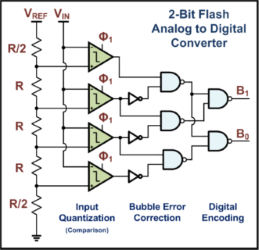
\includegraphics{ADCsch.png}}
\caption{Schematic for a simple 2-bit Flash ADC.}
\end{figure}

\begin{figure}[htbp]
\centerline{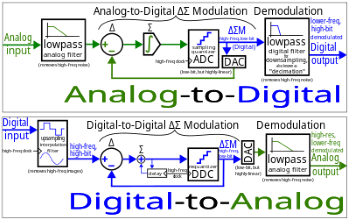
\includegraphics{ADCschDS.png}}
\caption{Schematic for a complex Delta-Sigma ADC.}
\end{figure}

\section{Working Principle}

The key parameters of an ADC to watch for include but are not limited to:

\begin{itemize}
    \item DC offset error. When the output deviates from the ideal value due to a shift in the input-output transfer function.
    \item DC gain error. When the slope of the actual transfer function deviates from the ideal slope, which is determined by the full-scale range and the number of bits.
    \item signal-to-noise ratio (SNR). The ratio of the power of the input signal to the power of the noise that is present in the output.
    \item Total harmonic distortion (THD). The distortion caused by the nonlinearity of an ADC.
    \item Integral nonlinearity (INL). The deviation of the actual transfer function from the ideal linear and uniform one.
    \item Differential nonlinearity (DNL). The deviation of the actual output step size from the ideal value.
    \item Spurious free dynamic range. The ratio of the power of the input signal to the power of the strongest spurious signal in the output.
    \item Power dissipation. The amount of energy that is consumed or lost during the conversion process.
\end{itemize}

On the supplied datasheet of TLC5540, Texas Instruments provides the recommended configuration of it in a circuit as seen in Fig. 5.

\begin{figure}[htbp]
\centerline{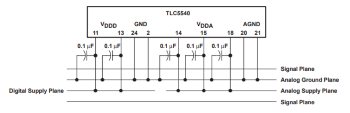
\includegraphics{ADCchipconfig.png}}
\caption{The recommended configuration of the TLC5540.}
\end{figure}

\section{Discussions}

\subsection{Advantages of ADCs}
\begin{itemize}
    \item Allows digital circuits to interface with the real world by encoding physical quantities such as sound, light, temperature, or movement into binary data 1 \cite{b3}.
    \item Enables complex processing and manipulation of analog signals using digital techniques, such as filtering, compression, encryption, or modulation \cite{b4}.
    \item Reduces the effects of noise and interference on analog signals, as digital signals are more robust and can be restored using error correction methods \cite{b5}.
\end{itemize}

\subsection{Disadvantages of ADCs}

One Disadvantage of ADCs are that they introduces quantization error and noise in the conversion process. This is because the analog signal is approximated by a finite number of discrete levels, thus some outputs are approximated. \par
Another disadvantage is that due to the inherent complexity of the design, they consume more power and area than analog circuits. This is because it involves multiple components such as comparators, encoders, and registers. \par
Some also suffer from nonlinearity, offset, and gain errors due to the mismatch and variation of the ADC components.

\subsection{Current Limitations}

A current limitation of ADCs today is quantization error. The higher the number of bits, the lower the quantization error, but also the higher the power consumption and cost of the ADC \cite{b6}. \par
Another limitation is sampling rate. The higher the sampling rate, the higher the bandwidth and resolution of the ADC, but also the higher the power consumption and complexity of the ADC \cite{b3}. \par
A rare but unfortunate limitation is conversion error. Conversion produces an incorrect output that is outside its normal function. This kind of error can degrade the reliability and quality of the ADC, and can be detected and corrected by using techniques such as error correction codes and calibration methods \cite{b7}.

\section{Conclusion}

For this research, I chose the 8-bit ADC TLC5540 from Texas Instruments.
I chose the TLC5540 because I had recently built a 3-bit Flash ADC for the final project in ECE 715. This made it was easier to carry over information between this report and that report as well as deepening my knowledge in ADCs overall.
The goal of this project was to explore the potential applications of the TLC5540 ADC in various fields, such as digital signal processing, data acquisition, and communication systems.

\begin{thebibliography}{00}
\bibitem{b1} 8-Bit, 40-MSPS Analog-to-Digital Converter (ADC), TLC5540, Rev. D, Texas Intruments, 2004, https://www.ti.com/lit/ds/symlink/tlc5540.pdf
\bibitem{b2} History of Analog-to-Digital Converters (ADCs), Data Acquisition | Test and Measurement Solutions, https://dewesoft.com/blog/history-of-analog-to-digital-converters
\bibitem{b3} Analog to Digital Converter (ADC); Advantages \& Disadvantages, Electricalvoice, https://electricalvoice.com/analog-to-digital-converter-adc-advantages/
\bibitem{b4} Electronics Tutorials, Analogue to Digital Converter (ADC) Basics, Basic Electronics Tutorials, 2020, https://www.electronics-tutorials.ws/combination/analogue-to-digital-converter.html
\bibitem{b5} Analog to Digital Converter : Block Diagram, Types \& Its Applications, ElProCus - Electronic Projects for Engineering Students, 2014, https://www.elprocus.com/analog-to-digital-converter/
\bibitem{b6} The limitations of the ADC, jeelabs.org, 2016, https://jeelabs.org/article/1614a/
\bibitem{b7} I. Beavers, Demystifying the Conversion Error Rate of High Speed ADCs, Analog.com, 2014, https://www.analog.com/en/technical-articles/demystifying-the-conversion-error-rate-of-high-speed-adcs.html
\end{thebibliography}

\end{document}
